% \subsection{Motivation}

\begin{frame}{Multi-Spectral Imaging}
  \begin{itemize}
    \item Multiple channels, small bandwidths.
    \item Enables spectral un-mixing (precision agriculture).
    \item Our focus: thermal spectrum ($7-14 \mu m$). 
    \item Cons: Expensive.
  \end{itemize}

  \begin{figure}
    \centering
    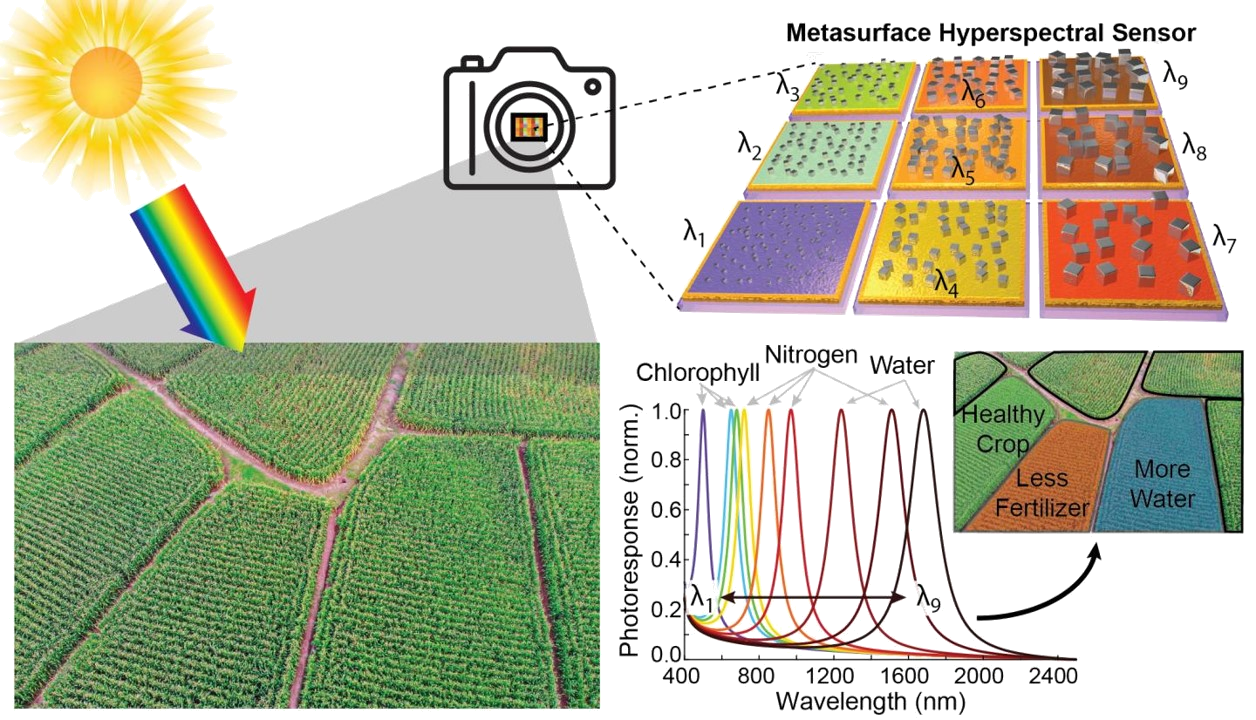
\includegraphics[width=0.6\linewidth]{../figs/introduction/multispectral.png}
  \end{figure}  
\end{frame}

\begin{frame}{Alternative}
    \begin{itemize}
      \item Simpler sensor (cost reduction).
      \item Compensate for compromised quality with CV algorithms.
      \item Deep learning (DL) techniques achieve state-of-the-art (SOTA) results.
      \item Issue: no multispectral thermal data.
    \end{itemize}
  
    \begin{figure}
      \centering
      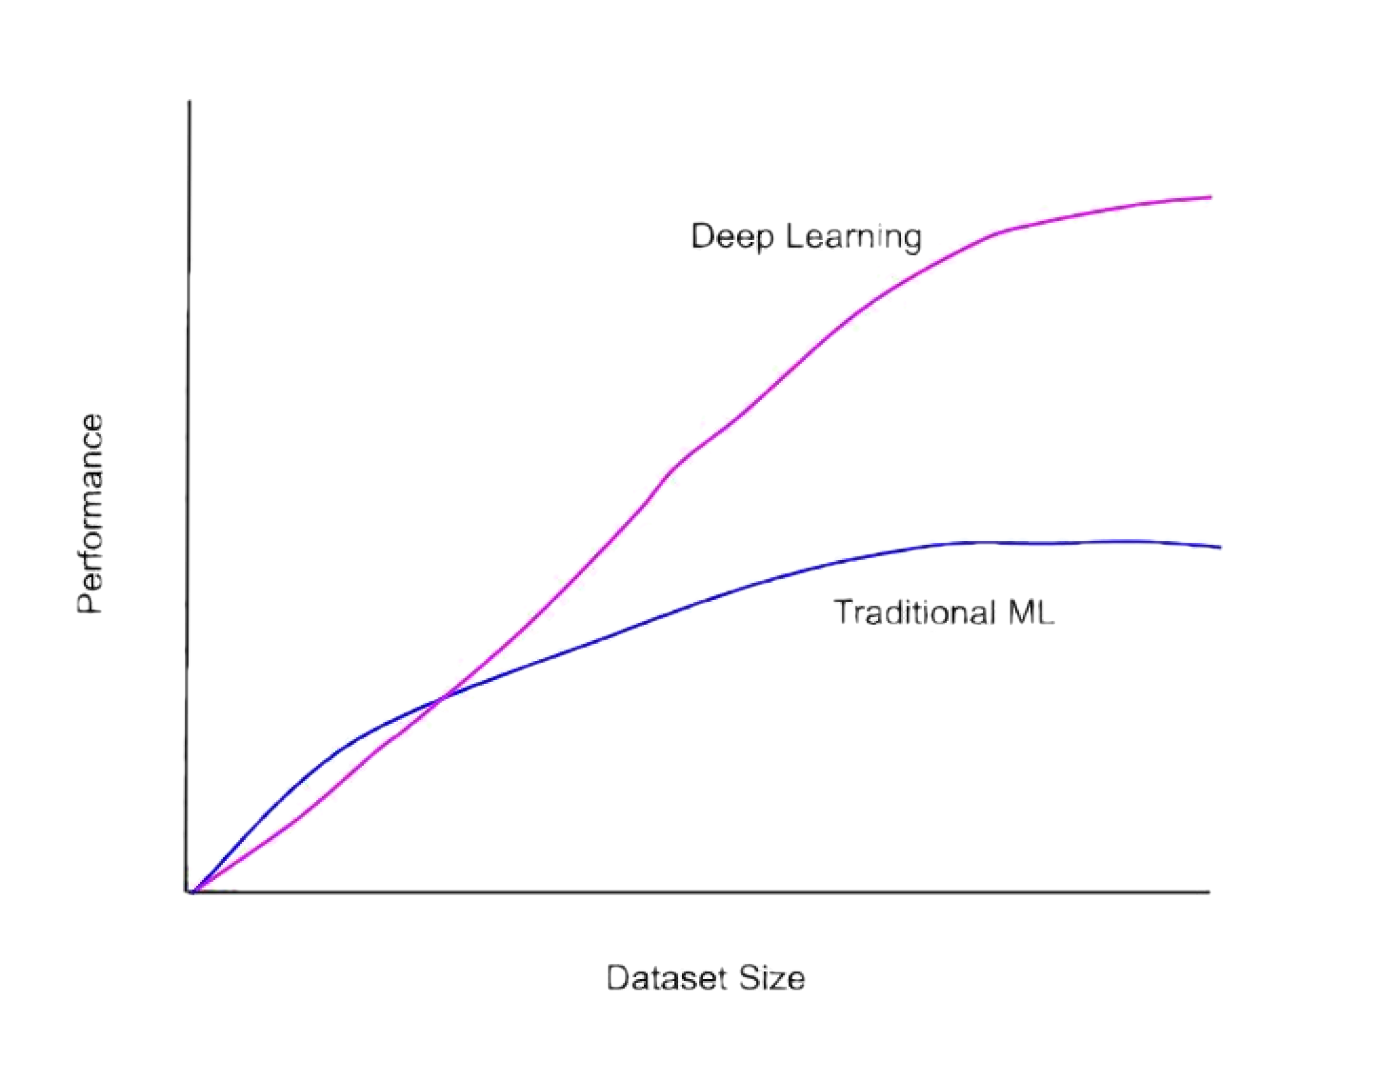
\includegraphics[width=0.5\linewidth]{../figs/introduction/dl_data_requirement.png}
    \end{figure}
  \end{frame}

\begin{frame}{Data Collection}
  \begin{itemize}
        \item Lightweight airplane.
        \item Several flights, each with some IR filter (monochromatic) or without (panchromatic). \hyperlink{apndx:data_collection}{\beamerbutton{More details}}
        \item Issues: registration, small sample size.
    \end{itemize}
    \begin{figure}
        \centering
        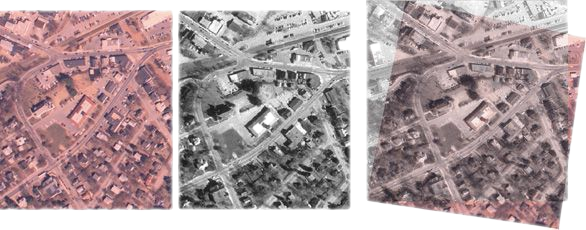
\includegraphics[width=0.8\linewidth]{../figs/introduction/registration.png}
      \end{figure}
  \end{frame}

\begin{frame}{Unpaired Image to Image (UI2I) Generative Models}
  \begin{itemize}
    \item Circumvents the need for \texttt{\textbraceleft} input, target \texttt{\textbraceright} tuples.
    \item Spatially consistent transformation between different modalities.
    \begin{figure}
      \centering
      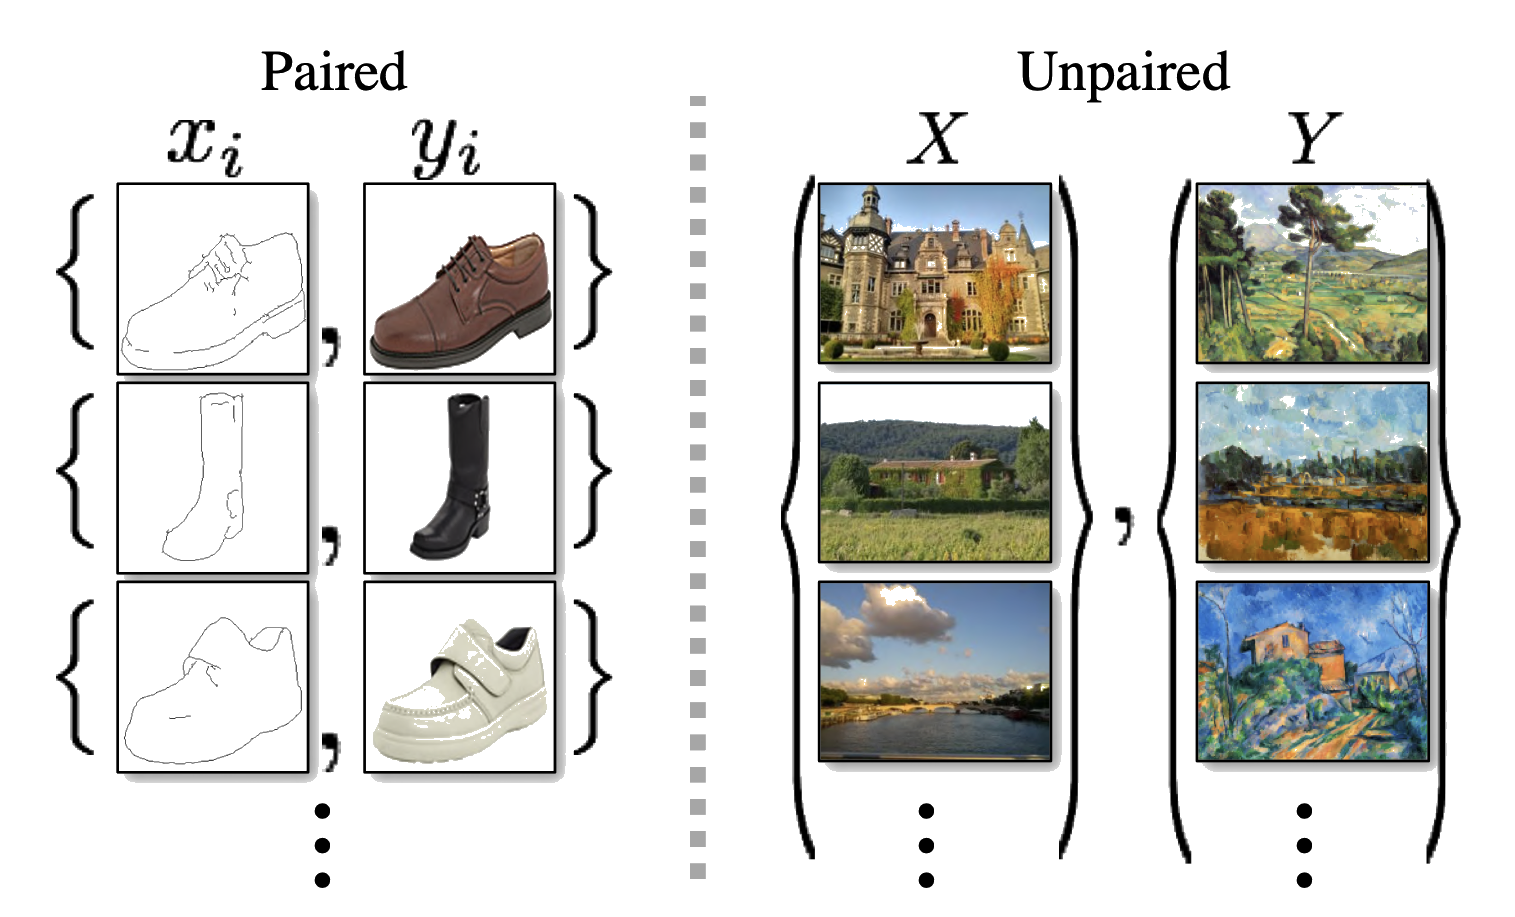
\includegraphics[width=0.7\linewidth]{../figs/related_work/paird_vs_unpaired_I2I.png}
    \end{figure}
  \end{itemize}
\end{frame}

\begin{frame}{Research Motivation}
  \begin{exampleblock}{Goal}
    Learn an UI2I transformation between different thermal spectra.
  \end{exampleblock} 
  \begin{exampleblock}{Hypothesis}
    Unique thermal physics can improve the quality of deep UI2I models.
  \end{exampleblock}  
  \begin{exampleblock}{Showcase}
    Transformation of wide-band (panchromatic) thermal images and to narrow-band (monochromatic) thermal images.
  \end{exampleblock}
\end{frame}